\section{Implementation}

To make a design decision, we must re-evaluate our functional requirements based off of the techniques gleaned and the lessons learnt from Background and Related Work.

The main choice we face is whether to use dynamic or static detouring. Even though implementing detouring at runtime offers advantages such as flexibility and ease of development, we must rule it out as an option because we have yet to find a dynamic method which does not compromise \emph{(F6)}. That is, all the runtime methods we have looked at require some form of environment, whether this is through the distribution of a shared library or otherwise. Deeming all dynamic solutions infeasible narrows down our options to the various static approaches.

\begin{figure}[H]
 \centering
 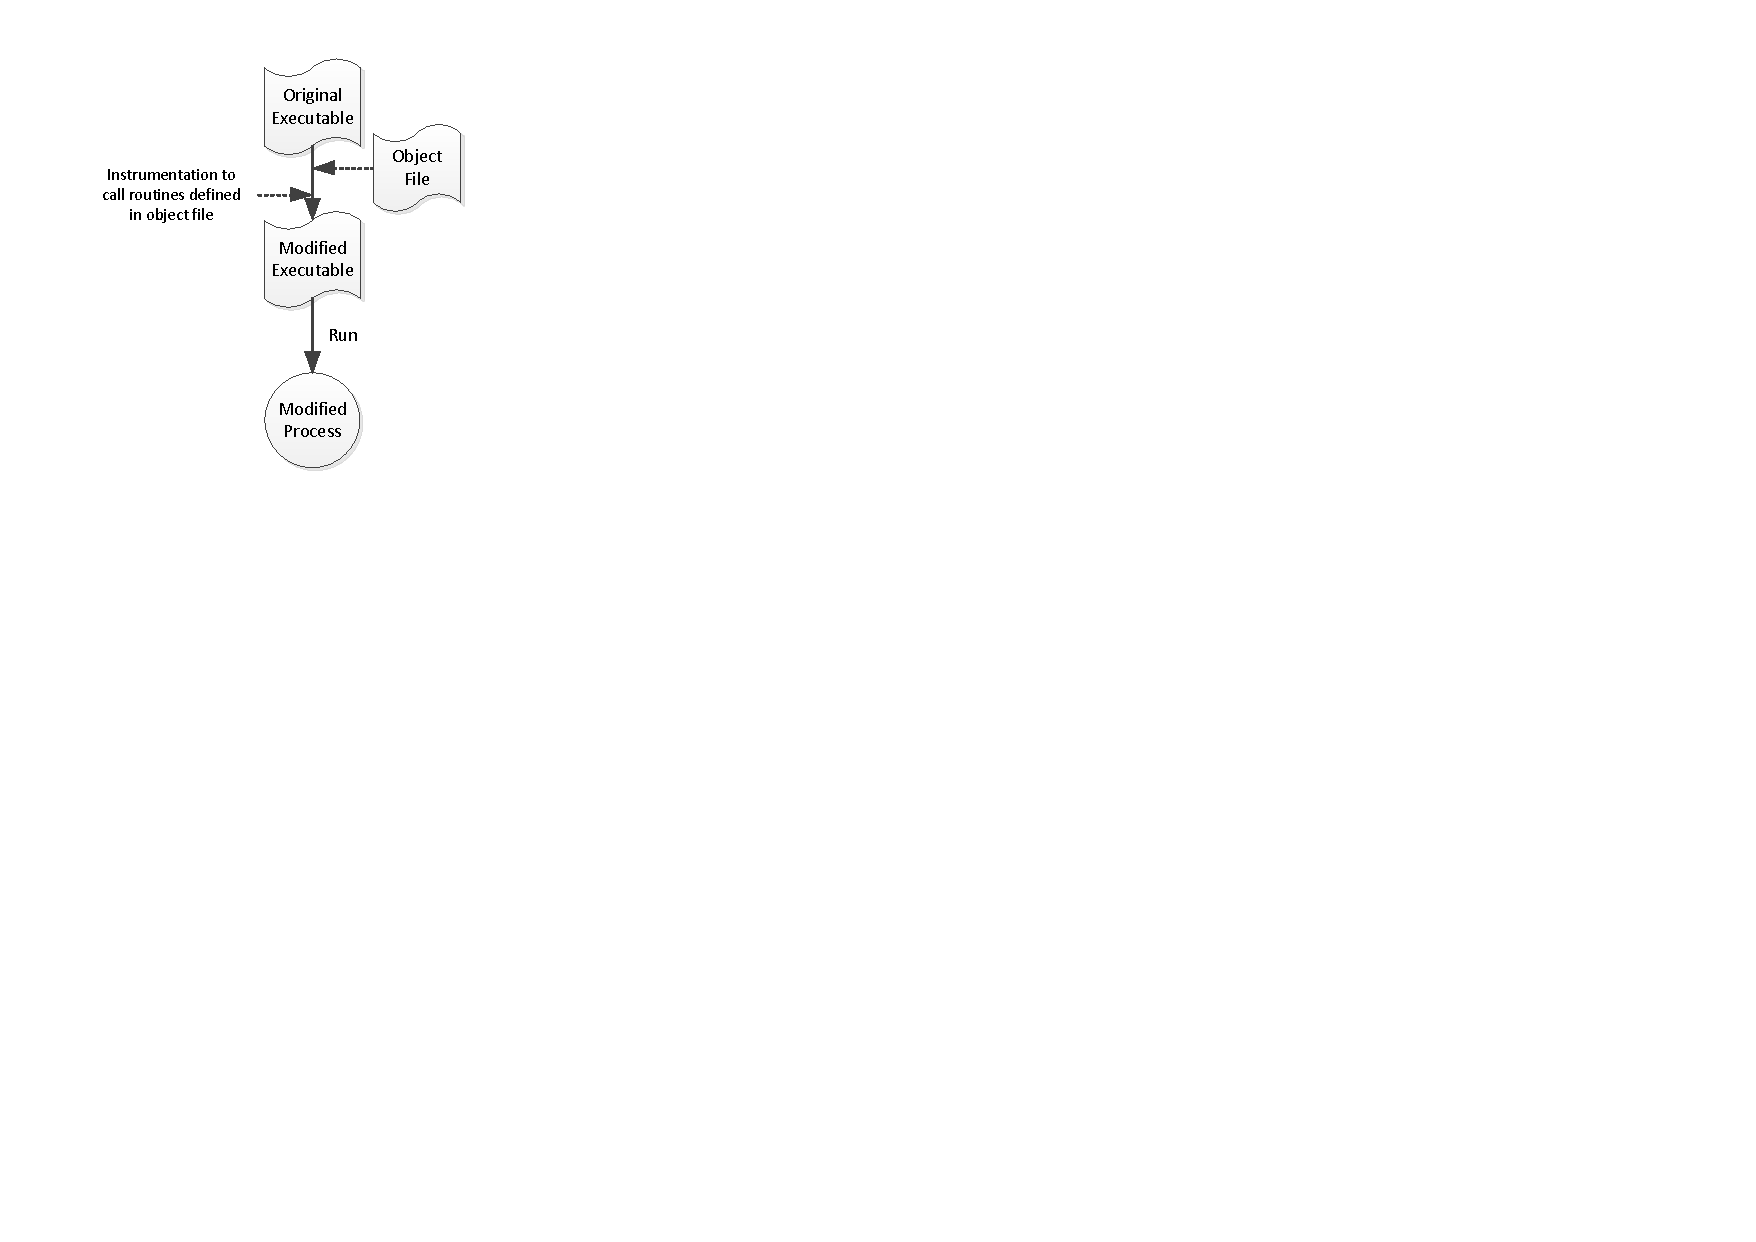
\includegraphics[viewport=49 370 223 569]{Workflow.pdf}
 \caption[Hierarchy]{The suggested method for instrumentation}
\end{figure}

We suggest an implementation of executable editing which works on top of the BFD library. This makes adaquate use of existing functionality as required by \emph{(F7)}. BFD will work in conjunction with the opcodes library to produce the control flow graph as required by \emph{(F4)} and \emph{(F5)}. To inject user-defined routines, we can take a similar approach to EEL and allow the user to specify an object file to be merged with the target binary. The next step would then be to find some mechanism by which procedural-level detouring can be achieved \emph{(F1)}. This is the first point at which we are modifying the target's code in any way. The technique used will have to be modified slightly to accommodate for the trampolining as required by \emph{(F2)}. Since the user defined functions are compiled separately to the target, they do not know what address to call for the trampoline so this is something we will have to deal with.

\section{Project Plan}

In order to complete the project, we need to satisfy all of the functional requirements. Given that we already have some form of plan for the implementation of the library, we can come up with some milestones and an approximate timeline:

\begin{table}[H]
 \caption{Projected timetable for project}
 \begin{tabular}{l p{12cm} }
 \hline
 Expected By & Milestone \\
 \hline
 Mid-Feb & Be able to perform static analysis of a program to generate the CFG \\
 End-Feb & Be able to inject an object file into targets \\
 End-Mar & Be able to perform regular detouring \\
 Mid-Apr & Be able to perform trampolining \\
 End-Apr & Perform evaluation and write user guide\\
 End-May & Write up the rest of the report \\
 \hline
 \end{tabular}
\end{table}

\subsection{Extensions}

If time permits, the most desirable extension is to add dynamic detouring to the library. We would implement some form of runtime detouring and provide users with the option to choose between both methods. Another smaller extension which would also be useful is to allow the library to be invocable through the command-line as well as through the API (as seen with ELFsh).